\documentclass{article}
\usepackage[utf8]{inputenc}
\usepackage{amsmath}
\usepackage{amsfonts}
\usepackage{amssymb}
\usepackage[cm]{fullpage}
\usepackage{hyperref}
\usepackage{enumitem}
\usepackage{array}
\usepackage{graphicx}
\usepackage{caption}
\usepackage{subcaption}
\usepackage{float}
\usepackage{moreverb}
\setdescription{labelindent=\parindent}
%%%%%%%%%%%%%%%%%%%%%%%%%%%%%%%%%%%%%%%%%
% Code Snippet
% LaTeX Template
% Version 1.0 (14/2/13)
%
% This template has been downloaded from:
% http://www.LaTeXTemplates.com
%
% Original author:
% Velimir Gayevskiy (vel@latextemplates.com)
%
% License:
% CC BY-NC-SA 3.0 (http://creativecommons.org/licenses/by-nc-sa/3.0/)
%
%%%%%%%%%%%%%%%%%%%%%%%%%%%%%%%%%%%%%%%%%
%----------------------------------------------------------------------------------------

\usepackage{listings} % Required for inserting code snippets
\usepackage[usenames,dvipsnames]{color} % Required for specifying custom colors and referring to colors by name

\definecolor{DarkGreen}{rgb}{0.0,0.4,0.0} % Comment color
\definecolor{highlight}{RGB}{255,251,204} % Code highlight color

\lstdefinestyle{Octave}{ % Define a style for your code snippet, multiple definitions can be made if, for example, you wish to insert multiple code snippets using different programming languages into one document
language=Octave, % Detects keywords, comments, strings, functions, etc for the language specified
%backgroundcolor=\color{highlight}, % Set the background color for the snippet - useful for highlighting
backgroundcolor=\color{white}, % Set the background color for the snippet
basicstyle=\footnotesize\ttfamily, % The default font size and style of the code
breakatwhitespace=false, % If true, only allows line breaks at white space
breaklines=true, % Automatic line breaking (prevents code from protruding outside the box)
captionpos=b, % Sets the caption position: b for bottom; t for top
commentstyle=\usefont{T1}{pcr}{m}{sl}\color{DarkGreen}, % Style of comments within the code - dark green courier font
deletekeywords={}, % If you want to delete any keywords from the current language separate them by commas
%escapeinside={\%}, % This allows you to escape to LaTeX using the character in the bracket
firstnumber=1, % Line numbers begin at line 1
frame=single, % Frame around the code box, value can be: none, leftline, topline, bottomline, lines, single, shadowbox
frameround=tttt, % Rounds the corners of the frame for the top left, top right, bottom left and bottom right positions
keywordstyle=\color{Blue}\bf, % Functions are bold and blue
morekeywords={}, % Add any functions no included by default here separated by commas
numbers=left, % Location of line numbers, can take the values of: none, left, right
numbersep=10pt, % Distance of line numbers from the code box
numberstyle=\tiny\color{Gray}, % Style used for line numbers
rulecolor=\color{black}, % Frame border color
showstringspaces=false, % Don't put marks in string spaces
showtabs=false, % Display tabs in the code as lines
stepnumber=5, % The step distance between line numbers, i.e. how often will lines be numbered
stringstyle=\color{Purple}, % Strings are purple
tabsize=2, % Number of spaces per tab in the code
}
\lstdefinestyle{Python}{ % Define a style for your code snippet, multiple definitions can be made if, for example, you wish to insert multiple code snippets using different programming languages into one document
language=Python, % Detects keywords, comments, strings, functions, etc for the language specified
%backgroundcolor=\color{highlight}, % Set the background color for the snippet - useful for highlighting
backgroundcolor=\color{white}, % Set the background color for the snippet
basicstyle=\footnotesize\ttfamily, % The default font size and style of the code
breakatwhitespace=false, % If true, only allows line breaks at white space
breaklines=true, % Automatic line breaking (prevents code from protruding outside the box)
captionpos=b, % Sets the caption position: b for bottom; t for top
commentstyle=\usefont{T1}{pcr}{m}{sl}\color{DarkGreen}, % Style of comments within the code - dark green courier font
deletekeywords={}, % If you want to delete any keywords from the current language separate them by commas
%escapeinside={\%}, % This allows you to escape to LaTeX using the character in the bracket
firstnumber=1, % Line numbers begin at line 1
frame=single, % Frame around the code box, value can be: none, leftline, topline, bottomline, lines, single, shadowbox
frameround=tttt, % Rounds the corners of the frame for the top left, top right, bottom left and bottom right positions
keywordstyle=\color{Blue}\bf, % Functions are bold and blue
morekeywords={}, % Add any functions no included by default here separated by commas
numbers=left, % Location of line numbers, can take the values of: none, left, right
numbersep=10pt, % Distance of line numbers from the code box
numberstyle=\tiny\color{Gray}, % Style used for line numbers
rulecolor=\color{black}, % Frame border color
showstringspaces=false, % Don't put marks in string spaces
showtabs=false, % Display tabs in the code as lines
stepnumber=5, % The step distance between line numbers, i.e. how often will lines be numbered
stringstyle=\color{Purple}, % Strings are purple
tabsize=2, % Number of spaces per tab in the code
}

% Create a command to cleanly insert a snippet with the style above anywhere in the document
\newcommand{\insertcodeOctave}[2]{\begin{itemize}\item[]\lstinputlisting[caption=#2,label=#1,style=Octave]{#1}\end{itemize}} % The first argument is the script location/filename and the second is a caption for the listing
\newcommand{\insertcodePython}[2]{\begin{itemize}\item[]\lstinputlisting[caption=#2,label=#1,style=Python]{#1}\end{itemize}} % The first argument is the script location/filename and the second is a caption for the listing
% End Code Snippet
%%%%%%%%%%%%%%%%%%%%%%%%%%%%%%%%%%%%%%%%%
% Vector shortcuts
\newcommand*{\X}{\Vec{x}}
\newcommand*{\Y}{\Vec{y}}
\newcommand*{\Z}{\Vec{z}}
\newcommand*{\0}{\Vec{0}}
\newcommand*{\norm}[1]{\lVert#1\rVert_2}
% Greek shortcuts
\newcommand*{\al}{\alpha}
\newcommand*{\be}{\beta}
\newcommand*{\de}{\delta}
\newcommand*{\De}{\Delta}
\newcommand*{\ep}{\epsilon}
\newcommand*{\ga}{\gamma}
\newcommand*{\la}{\lambda}
\newcommand*{\om}{\omega}
%\newcommand*{\the}{\theta}
\begin{document}
\title
{\begin{flushleft}
\large
Patrick Pegus\\
Mini Project 3\\
\today\\
CMPSCI-689\\
Prof. Sridhar Mahadevan
\end{flushleft}}
\author{}
\date{}
\maketitle
\normalsize
\begin{enumerate}
	\item
		\begin{enumerate}
			\item
				\begin{align*}
					w_{FP}
					&= argmin_w \left\| \Pi_\Phi T^\pi(\hat{V}) -\hat{V} \right\| \\ \nonumber
					&= argmin_w \left\| \Pi_\Phi \left(R^\pi + \ga P^\pi \Phi w\right) -\Phi w \right\|
				\end{align*}
				The norm is minimized if
				\begin{align*}
					\Phi w &= \Pi_\Phi \left(R^\pi + \ga P^\pi \Phi w\right) \\
					\Phi w &= \Phi\left(\Phi^T \Phi\right)^{-1}\Phi^T \left(R^\pi + \ga P^\pi \Phi w\right) \\
					w &= \left(\Phi^T \Phi\right)^{-1}\Phi^T \left(R^\pi + \ga P^\pi \Phi w\right) \\
					w &= \left(\Phi^T \Phi\right)^{-1}\Phi^T R^\pi + \ga \left(\Phi^T \Phi\right)^{-1}\Phi^T P^\pi \Phi w \\
					w - \ga \left(\Phi^T \Phi\right)^{-1}\Phi^T P^\pi \Phi w &= \left(\Phi^T \Phi\right)^{-1}\Phi^T R^\pi \\
					\left(I - \ga \left(\Phi^T \Phi\right)^{-1}\Phi^T P^\pi \Phi\right)w &= \left(\Phi^T \Phi\right)^{-1}\Phi^T R^\pi \\
					w &= \left(I - \ga \left(\Phi^T \Phi\right)^{-1}\Phi^T P^\pi \Phi\right)^{-1}\left(\Phi^T \Phi\right)^{-1}\Phi^T R^\pi \\
					w &= \left(\left(\Phi^T \Phi\right) \left(I - \ga \left(\Phi^T \Phi\right)^{-1}\Phi^T P^\pi \Phi\right)\right)^{-1}\Phi^T R^\pi \\
					w &= \left(\Phi^T \Phi - \ga \Phi^T P^\pi \Phi\right)^{-1}\Phi^T R^\pi \\
					w &= \left(\Phi^T \left(\Phi - \ga P^\pi \Phi\right)\right)^{-1}\Phi^T R^\pi \\
					w &= \left(\Phi^T \left(I - \ga P^\pi \right)\Phi\right)^{-1}\Phi^T R^\pi \\
				\end{align*}
			\item
				\begin{align*}
					w_{LS}
					&= argmin_w \left\| T^\pi(\hat{V}) -\hat{V} \right\| \\
					&= argmin_w \left\| R^\pi + \ga P^\pi \Phi w -\Phi w \right\|
				\end{align*}
				The norm is minimized if
				\begin{align*}
					\Phi w - \ga P^\pi \Phi w = \left(I - \ga P^\pi\right) \Phi w  \approx R^\pi
				\end{align*}
				This is equivalent to a weighted least squares problem $Ax \approx b$, whose solution is $x = \left(A^T C A\right)^{-1} A^T C b$, where $C$ is a diagonal matrix with entries giving
				the non-uniform weights measuring the ``length'' in the space ~\cite{mahadevan}.
				Let $A = \left(I - \ga P^\pi\right) \Phi w$, $b = R^\pi$, and $C = I$, if the basis functions uniform importance.
				Therefore,
				\begin{align*}
					w
					&= \left(\left(\left(I - \ga P^\pi\right)\Phi\right)^T I \left(\left(I - \ga P^\pi\right)\Phi\right)\right)^{-1} \left(\left(I - \ga P^\pi\right)\Phi\right)^T I R^\pi \\
					&= \left(\Phi^T\left(I - \ga P^\pi\right)^T\left(I - \ga P^\pi\right)\Phi\right)^{-1} \Phi^T\left(I - \ga P^\pi\right)^T R^\pi
				\end{align*}
		\end{enumerate}
	\item
		\begin{enumerate}
			\item
				\begin{align*}
					\De_{\theta_i}L_i(\theta_i)
					&= \De_{\theta_i} E_{s,a\sim p(\cdot)}\left[\left(y_i - Q(s,a;\theta_i)\right)^2\right] \\
					&= -2E_{s,a\sim p(\cdot)}\left[\left(y_i - Q(s,a;\theta_i)\right)\De_{\theta_i}Q(s,a;\theta_i)\right] \\
					&= -2E_{s,a\sim p(\cdot)}\left[\left(E_{s'\sim\varepsilon}\left[\left.r + \ga\max_{a'}Q(s',a';\theta_{i-1})\right|s,a\right] - Q(s,a;\theta_i)\right)\De_{\theta_i}Q(s,a;\theta_i)\right] \\
					&= -2E_{s,a\sim p(\cdot)}\left[\left(\sum_{s'}\left[\left(r + \ga\max_{a'}Q(s',a';\theta_{i-1})\right)p(s')\right] - Q(s,a;\theta_i)\right)\De_{\theta_i}Q(s,a;\theta_i)\right] \\
					&= -2E_{s,a\sim p(\cdot)}\sum_{s'}\left[\left(\left(r + \ga\max_{a'}Q(s',a';\theta_{i-1})\right)p(s') - Q(s,a;\theta_i)\right)\De_{\theta_i}Q(s,a;\theta_i)\right] \\
					&= -2E_{s,a\sim p(\cdot);s'\sim\varepsilon}\left[\left(r + \ga\max_{a'}Q(s',a';\theta_{i-1}) - Q(s,a;\theta_i)\right)\De_{\theta_i}Q(s,a;\theta_i)\right] \\
				\end{align*}
				We can disregard the $-2$, since a constant multiplier will not affect when the gradient is $0$.
			\item TD-gammon approximated a value function for states instead of an action-value function approximation used in Deep Mind.
				Also, TD-gammon learnt this state value function on-policy, meaning that it follows an exploration policy.
				On the other hand, Deep Mind learnt about the greedy strategy of choosing the action with the greatest current value.
			\item
				Deep Mind uses experience replay to smooth the behavior distribution over many previously seen sequences.
				If experience replay was not used, then feedback loops could occur, meaning the behavior distribution could shift dramatically based on the most recent actions.
				These feedback loops may cause parameters choices that get stuck on poor local minima or diverge.
			\item
				The two left graphs show the average reward per episode vs. training epochs.
				For both Breakout and Seaquest, it is difficult to tell whether Deep Mind is creating more valuable policies with increased training time.
				In the two right graphs, they more directly measure this by showing the average action value vs. training epochs.
				Here we can see that the learning algorithm makes more consistent progress on Seaquest.
				%Although I am not familiar with either game, I suspect this may be because there is more non-determinism in Breakout than Seaquest.
		\end{enumerate}
	\item
		\begin{enumerate}
			\item
				\begin{figure}[H]
					\centering
					\caption{Average reward vs. learning rate.}
					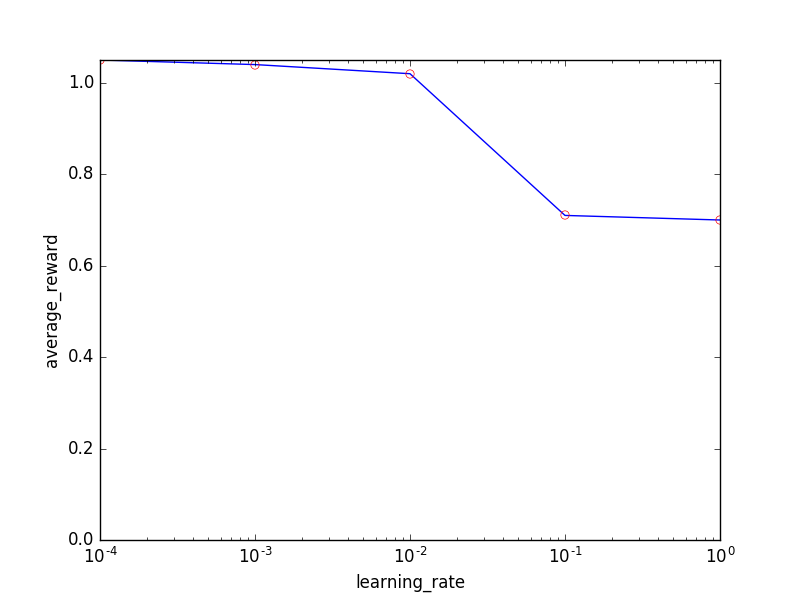
\includegraphics[width=0.5\textwidth]{fig/learning_rate.png}
					\label{fig:learning_rate}
				\end{figure}
				%http://cs.stanford.edu/people/karpathy/convnetjs/intro.html
				%The gradient is the vector in the parameter space along which your function (here probability of 4) increases the most. So we forwarded our image of 4, computed the probability of answer being 4, then computed the gradient on all parameters of the network, and finally we nudge all the parameters slightly along that gradient. Some people call this procedure backpropagation (or backprop), but in the form I presented it's also just stochastic gradient descent, a vanilla method in optimization literature.

				%The amount we nudge is called the learning rate, and is perhaps the single most important number in training these networks. If it's high, the networks learn faster, but if it's too high, the networks can explode. On the other hand, if it's too low the training will take a very long time. Usually you start it higher (for example say 0.1), but not too high (!) and anneal it slowly over time a few orders of magnitude (down to 0.0001 perhaps). 
				Generally, in Figure~\ref{fig:learning_rate} we see average reward increase as the learning rate or amount we move the parameters in the direction of the gradient decrease.
				However, as the learning rate decreased, the training time or the time it took the average reward to stabilize was substantially greater.
				No divergence in average reward occurred at the higher learning rates.
			\item
				\begin{figure}[H]
					\centering
					\caption{Average reward vs. momentum.}
					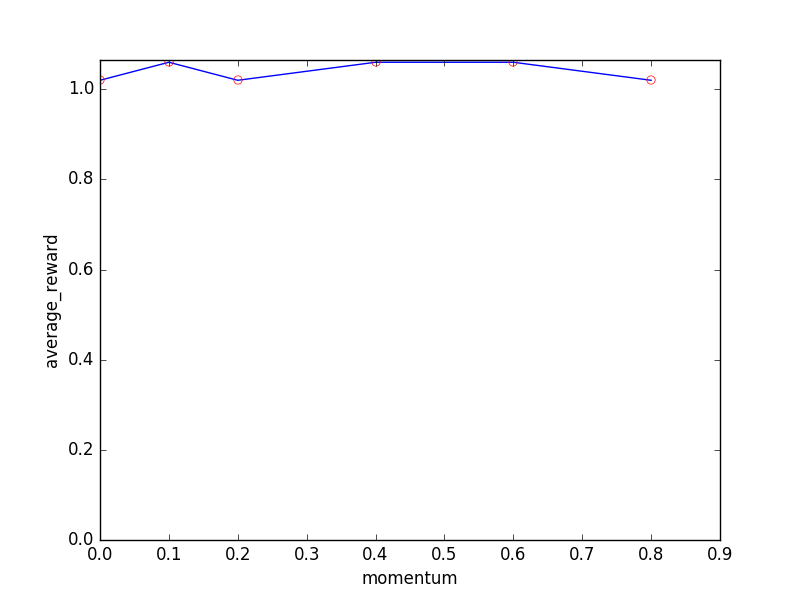
\includegraphics[width=0.5\textwidth]{fig/momentum.png}
					\label{fig:momentum}
				\end{figure}
				%http://ufldl.stanford.edu/tutorial/supervised/OptimizationStochasticGradientDescent/
				%If the objective has the form of a long shallow ravine leading to the optimum and steep walls on the sides, standard SGD will tend to oscillate across the narrow ravine since the negative gradient will point down one of the steep sides rather than along the ravine towards the optimum. The objectives of deep architectures have this form near local optima and thus standard SGD can lead to very slow convergence particularly after the initial steep gains. Momentum is one method for pushing the objective more quickly along the shallow ravine.
				%Above values had momentum = 0.
				%Using learning rate of 0.01.
				As Figure~\ref{fig:momentum} shows, changing the momentum had no visible effect on the average reward.
				This makes sense as increased momentum will at best force stochastic gradient descent to reach optimal values more quickly.
			\item
				\begin{figure}[H]
					\centering
					\caption{Average reward vs. discount factor.}
					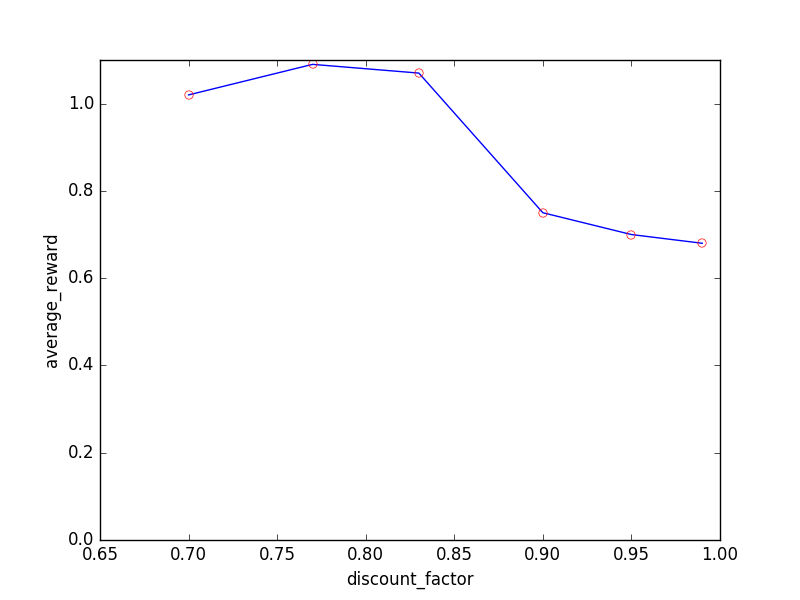
\includegraphics[width=0.5\textwidth]{fig/discount_factor.png}
					\label{fig:discount_factor}
				\end{figure}
				%discount factor originally 0.7, learning_rate 0.01, momentum 0
				%performance decreases as lambda increases meaning that a greedy strategy is better
				%this makes sense when looking at the graphic because there don't seem to be instances
				%in which the agent must eat poison in order to get many apples or 
				%alternatively eat avoid an apple in order to avoid eating a lot of poison
				Figure~\ref{fig:discount_factor} shows that average reward generally decreases as the discount factor increases.
				Therefore, the greedy strategy of maximizing the reward of short-term actions results in a more valuable policy.
				This agrees with the environment shown in the graphic.
				For instance, there don't seem to be instances in which the agent must eat poison in order to get many apples or alternatively avoid an apple in order to avoid eating a lot of poison.
			\item
				\begin{figure}[H]
					\centering
					\caption{Average reward vs. experience size.}
					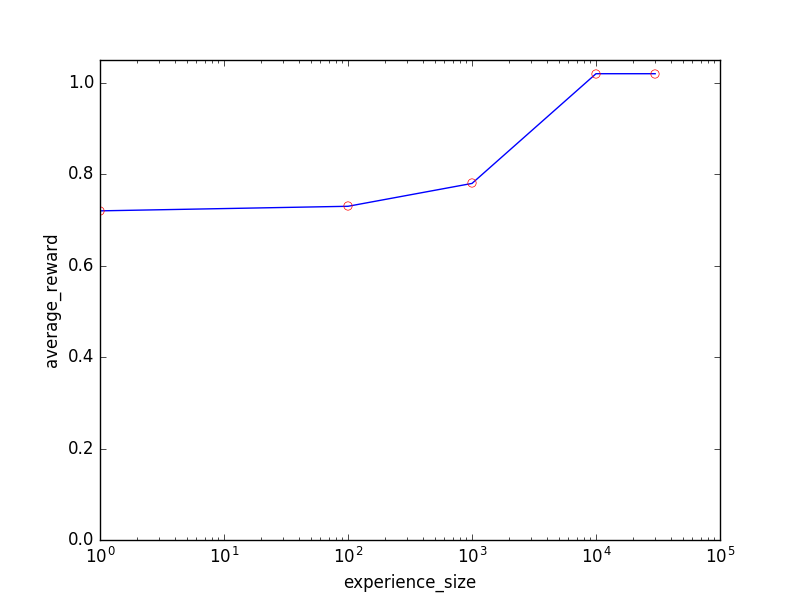
\includegraphics[width=0.5\textwidth]{fig/experience_size.png}
					\label{fig:experience_size}
				\end{figure}
				%experience size originally 30000
				%no divergence at 0
				As Figure~\ref{fig:experience_size} shows, increased replay memory size improved average reward, especially as the size reached 10000.
				With this implementation, there was no divergence with low memory size alluded to in \cite{deepmind}.
		\end{enumerate}
\end{enumerate}

\bibliographystyle{abbrv}
\bibliography{report}

\end{document}
